% Chapter 4 from the standard thesis template
% that contains an adv. example table and figure.

\section{Software Defined Radio Theory of Operation}


\subsection{Software Defined Power Detection}

A traditional radiometer uses a square-law detector which takes the input signal and produces a voltage that is proportional to the square of the voltage.  This allows us to take an analog RF signal and convert the noise voltage that for all intense and purposes has a mean value of zero, and produce a noise power.

For a SDR, the incoming signal is sampled and converted to I/Q values by the hardware within the SDR.  The I/Q values together can be used to recontruct both the phase, frequency and amplitude information of the signal and can do so much more accurately then if we just recorded the frequency and amplitude information.  In GNURadio we are then able to square these values within software which give us our peak voltage of the signal.  This block in GNURadio mathematically performs what is shown in equation \ref{sdr_x2}.

\begin{equation}\label{sdr_x2}
I^2+Q^2 = P_{out}
\end{equation}

Therefore, like the analog square-law detector we are taking peak voltage values, which has an equivalent noise voltage and a mean value of zero, and square them to produce a noise power that is proportional to the square of this amplitude.

Like the analog square-law detector, this signal will fluctuate rapidly and to improve the sensitivity of the radiometer we wish to integrate this signal.  We now want to look at how we can replicate a RC filter or integrator in the software defined radio.

\subsection{Software Defined Integrator}
A RC filter is analogous to an integrator where the R and C values determine our time constant and our integration time for the filter[\cite{Aitken}].  We know a RC filter is analogous to an integrator by looking at equation \ref{eq:rc_int}.  A SDR however operates in the digital domain at discrete intervals.  One type of filter that can be used is the Infinite Impulse Response (IIR) filter. 

\begin{equation}\label{eq:rc_int}
\frac{1}{RC}\int{V_idt}
\end{equation}


To begin with, we look at what an analog RC filter looks like. 

{\begin{figure}[h!tb] 
\centering
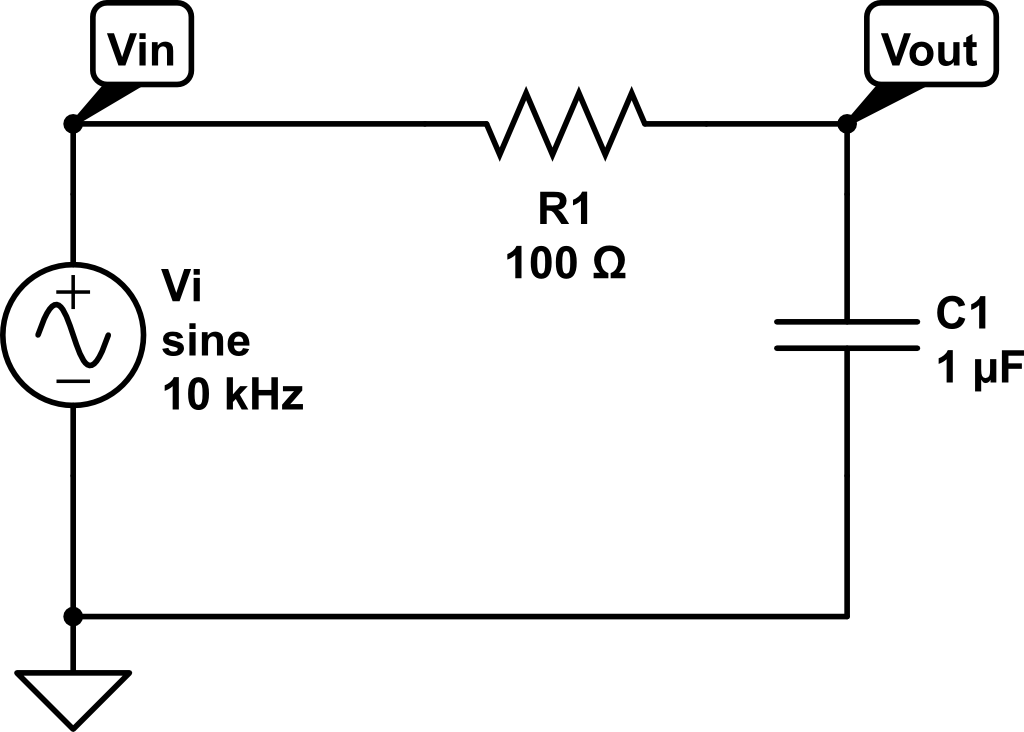
\includegraphics[width=10cm]{Images/rc-circuit.png}
\isucaption{A simple RC circuit}
\label{rc_circuit}
\end{figure}
}

This circuit can be represented by equation \ref{eq:rc_circuit_eq}.

\begin{equation}\label{eq:rc_circuit_eq}
\frac{V_{in}-V_{out}}{R}=C\frac{dV_{out}}{dt}
\end{equation}

A Finite Impulse Response (FIR) filter is a digital filter that can take an impulse signal and decays to zero after a finite number of iterations.  This type of digital filter can be represented by equation \ref{FIR_Eq} which mathematically expresses the FIR Filter.

\begin{equation}\label{FIR_Eq}
y_n=\displaystyle\sum\limits_{i=o}^{P-1} c_ix_{n-i}
\end{equation}

This simply says that the nth output is a weighted average of the most recent P inputs.  

An Infinite Impulse Response (IIR) filter is the same as the FIR filter, except that we add a summation term which feeds back the previous output.

\begin{equation}\label{IIR_eq}
y_n=\displaystyle\sum\limits_{i=o}^{P-1} c_ix_{n-i}+\displaystyle\sum\limits_{j=1}^{Q} d_jy_{n-j}
\end{equation}

Equation \ref{IIR_eq} shows that a FIR filter is a IIR filter, except that $Q=0$[\cite{Cross}].  

To get a better understanding on how the digital IIR filter relates to the RC filter analog, we can look at the Fourier Transform and the relationship of the input to the output in the frequency domain.

\begin{equation}\label{Fourier_IIR}
H(f)=\frac{\displaystyle\sum\limits_{j=o}^{P-1} c_je^{-2\pi ijfT}}{1-\displaystyle\sum\limits_{k=1}^{Q} d_ke^{-2\pi ikfT}}
\end{equation}

In equation \ref{Fourier_IIR}, $f$ is our frequency in Hz and $T$ is the time between samples in seconds and is related to our sampling frequency.

We now want to show the link between our analog RC circuit and the IIR filter.  Looking at equation \ref{eq:rc_circuit_eq}, which represents the differential equation relating the input voltage $V_{in}$ to the output voltage $V_{out}$, we can substitute for input and output of our IIR filter.  Since we are now in the time domain, we need to define what $T$ is and we can do that using equation \ref{sampling_rate_eq}.

\begin{equation}\label{sampling_rate_eq}
T=time between samples=\frac{1}{sampling rate}
\end{equation}

We can now relate our input voltage to the input to our IIR filter and the output voltage to the output of our IIR filter.

\begin{equation}\label{input_IIR}
x_n=v_{in}(nT)
\end{equation}

\begin{equation}\label{output_IIR}
y_n=v_{out}(nT)
\end{equation}

We can now rewrite our difference equation with $x_n$ and $y_n$.

\begin{equation}\label{diff_xn_yn}
\frac{x_n-y_n}{R}=C\frac{y_n-y_{n-1}}{T}
\end{equation}

Finally, we can solve for $y_n$ which results in our final equation for showing how a IIR filter is related to an RC filter.

\begin{equation}\label{final_IIR_RC}
y_n=\frac{T}{T+RC}x_n+\frac{RC}{T+RC}y_{n-1}
\end{equation}

It can be seen that an IIR filter can have the same frequency response as we expect from an analog RC filter.  As our sampling rate approaches infinity, the approximation gets closer to the original response from the analog RC circuit.  

For the cutoff frequency of a RC circuit, we know that it has the relationship shown in equation \ref{RC_relationship}.

\begin{equation}\label{RC_relationship}
f_c=\frac{\sqrt{3}}{2\pi RC}\rightarrow RC=\frac{\sqrt{3}}{2\pi f_c}
\end{equation}

The $RC$ term gives us our time constant of the circuit and can be used to calculate out our coefficients.  We are not concerned about the actual values of R and C with our IIR filter, instead we just need the product of R and C.  

In GNURadio most of the work is done for us.  We can simply enter in our desired cutoff frequency and GNURadio will calculate our IIR filter coefficients.  However, this shows that an IIR filter works much like an analog RC low pass filter.

Like a traditional radiometer, the SDR will use an antenna to look at the target of interest.  SDRs still use a RF stage that takes the power from the source and amplifies it.  The difference though begins after that.  A SDR will then sample and generate I and Q values that represents the amplitude and phase of the signal.  From there, this data is sent to a computer to be processed.  We can then use this information to calculate the power that is being seen.  In addition, we can manipulate the signal in other ways such as applying a filter to filter out an unwanted source.

\subsection{SDR Radiometer Summary}

As we have shown the two of the major components of a traditional radiometer, the power detection and integration of the signal can be replicated in software and therefore can be implemented in a software defined radio.  The information can now be stored, displayed or both for further analysis.  

There is one component of the software defined radio that we are not able to implement in software and that is with the signal amplification.  This however does play a major role in the performance of the radiometer and is a key element that should not be overlooked.  While this is not implemented in software, it still plays a critical role in our software defined radio radiometer. 

\subsection{RF Front End}

Hardware with a software defined radio still plays a critical role.  A traditional software defined radio will focus on digitizing the signal as soon as possible and the hardware used will be focused on performing that critical digitizing process.  For a software defined radio radiometer, we still want to digitize as soon as possible, but we also need to consider our noise factor.  Most software defined radios are designed for communication purposes such as implementing 802.11b or other wireless protocols.  In these scenarios a higher noise factor is not as detrimental to the overall system as it is with a radiometer.  This is because we have a known signal that is magnitudes greater than the noise floor.  In a radiometer however, we do not have this large separation between the information we need and the noise of the system.  And so our noise factor is a more critical component.  

To counter this, we use Low Noise Amplifiers to amplify the signal but it can also help lower our noise factor.  The first LNA in the chain contributes a large amount to our noise factor, so by selecting a LNA that has a low noise factor, it reduces the noise factor for the system.  This can be shown by looking at the equation that calculates our noise factor.

\begin{equation}\label{noise_factor}
F=F_1+\frac{F_2-1}{G_1}+\frac{F_3-1}{G_1 G_2}+\frac{F_4-1}{G_1 G_2 G_3}+\cdots +\frac{F_n-1}{G_1 G_2 G_3 \cdots G_{n-1}}
\end{equation}

While additional components do add to the noise figure, their contribution is significantly lower than the first LNA put in the RF chain.

This however is the only major change we need to do for doing radiometer work with an off the shelf radiometer.  The rest will be done within software which is the principal reason for using a software defined radio.

\section{General Specifications}
In general, since we are digitizing the signal early in the RF signal chain, the noise figure of the RF components in the SDR do not add a significant amount of noise to the system.  Additional performance metrics that require examination include how much bandwidth the system can handle.   The information below outlines the specification of the devices used and its impact on the performance of the SDR as a digital radiometer.   

\section{Comparison of a Software Defined Radio Radiometer vs Traditional Radiometer}

As outlined above, a software defined radio implements a traditional radiometer but in the digital domain.  For power detection, we simply sum the squares of the I and Q values that have been sampled by the software defined radios analog to digital converters.  As with a traditional radiometer, we also want to filter this information to remove much of the jitters that comes from the rapid fluctuations in the power readings.  This is done using an IIR low pass filter, which mimics a traditional RC low pass filter.  Once completed, we now have the total power reading from the radiometer and we can now store, display or do both with this information.  

A traditional radiometer may also use an analog to digital converter in order to digitize the analog voltage from the square-law detector.  Because the sample rate of this voltage is low, almost any analog to digital can be used for this.  At this point however, there is no frequency information, only the magnitude information is being retained and recorded.
